\section{Prüfung 17.11.2021}
\subsection{Echtzeit}
\subsubsection{a)}
Ein Profit/Penalty-Diagramm gibt den Nutzen bzw. den Schaden der Ausfuhrung einer Operation als 
kontinuierlichen Zahlenwert in Abhangigkeit vom Zeitpunkt der Ausifihrung an Positive Werte 
bedeuten einen Nutzen, negative einen Schaden — je größer der Absolutwert, desto größer der Nutzen bzw. der Schaden. 
Ein Fahrzeug benotigt 10 Sekunden zum Uberqueren einer Kreuzung mit einer Ampel. 
Zeichnen Sie in das folgende Diagramm den Profit/Penalty-Verlauf fOr die Operation „Fahrzeug fahrt in Kreuzung ein" 
für den Fall dass die Ampel zunächst 50 Sekunden Grün zeigt, dann 20 Sekunden Gelb and dann 50 Sekunden Rot. 

\begin{figure}[H]
  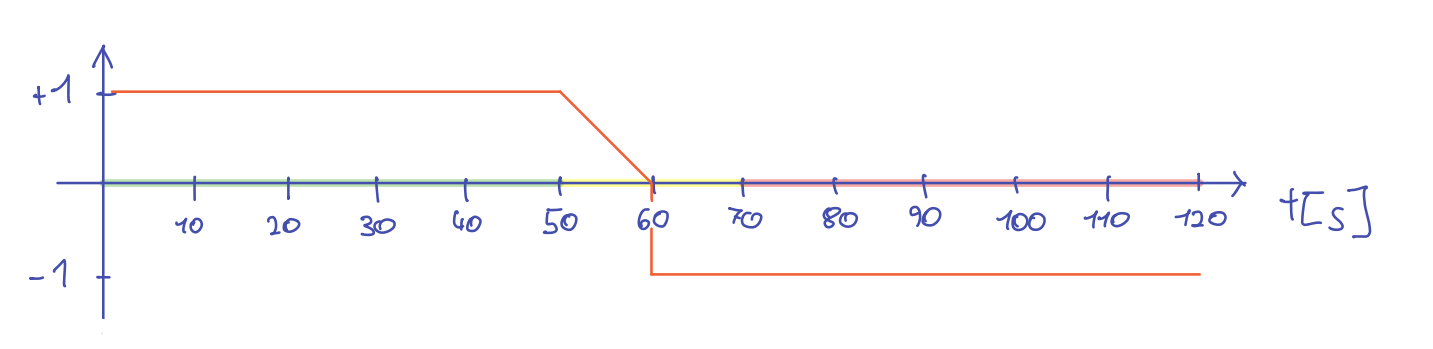
\includegraphics[width=10cm]{images/KA171121/1a.png}
  \centering
\end{figure}

\subsubsection{b)}
Handelt es sich hier um weiche, feste oder harte Echzeit? Begründen Sie!

Es handelt sich um harte Echtzeit, fährt das Auto zu spät in die Kreuzung ein kann es zu einem Schaden durch 
andere Autos kommen. Hier muss angenommen werden, dass wenn Rot aufleuchtet andere Autos schon wegfahren und 
nicht auf Autos in der Kreuzung achten.

\subsection{Busse}
\subsubsection{a)}
Warum ist Standard-Ethernet nicht echtzeitfähig?

Standard-Ethernet vewendet CSMA/CD und TCP/IP welche dieses Methode nicht echtzeitfähig macht. Es werden
Kollisionen detektiert. Gibt es eine Kollision wird eine zufällige Zeit gewartet und das Paket erneut angefordet.

\subsubsection{b)}
Was versteht man unter Arbitrierung und wie ist diese beim CAN-Bus realisiert?

Bus Arbitrierung bedeuted, dass immer nur eine Kommunikation zugleich stattfinden kann (alle nacheinander $\rightarrow$ bottleneck).
Arbitrierung entscheided wer senden darf.

All masters send identifiers at the same time. If a node hears a dominant bit
but sends it recessively, it withdraws, i.e. the message with the smallest
identifier has the highest priority (00...0) (see I2C bus).
CSMA/AMP: Carrier Sense Multiple Access with Arbitration on Message
Priority\footnote{Folien Kap2\_3 S47}

\subsubsection{c)}
Zwei I2C-Master sind mit einem gemeinsamen I2C-Bus verbunden und versuchen gleichzeitig Daten an einen ebenfalls 
mit dem Bus verbundenen I2C-Slave zu senden. Die Adresse des Slave ist Ox2A (7-Bit Adresse) und das Register in 
welches geschrieben wird ist 0x36. Nehmen Sie an, dass der erste Master die Nutzdaten 0x71 und der zweite Master 
die Nutzdaten 0x72 in das Register schreibt. Welche Symbol-Folge wird über die SDL-Leitung des I2C-Buses gesendet? 
Die folgenden Symbole werden dabei verwendet: 

\begin{itemize}
  \item 0 für Bit 0
  \item 1 für Bit 1
  \item S für das Start-Signal
  \item P für das Stopp-Signal
  \item A für das ACK-Bit
\end{itemize}
Slave 0x2a = 010 1011\\
Register 0x36 = 0011 0110\\
Master1 0x71 = 0111 0001\\
Master2 0x72 = 0111 0010\\

Master1 sendet als erstes da Nutzdaten von Master1 $<$ Master2 ist
\begin{equation}
  S\underbrace{0101011}_{Slave addr}\underbrace{0}_{R/N}A\underbrace{00110110}_{Register addr}\underbrace{01110001}_{payload}AP
\end{equation}

anschließend sendet Master2

\begin{equation}
  S\underbrace{0101011}_{Slave addr}\underbrace{0}_{R/N}A\underbrace{00110110}_{Register addr}\underbrace{01110010}_{payload}AP
\end{equation}


\subsection{Echzeitscheduling}
Bestimmen Sie (ohne Zeichnen) für die unten gegebenen Tasks die Schedulebarkeit mit RMS und EDF in Abhängigkeit vom 
Parameter n und geben Sie in der Tabelle unten an für welche Werte von n die Tasks mit RMS bzw. EDF auf jeden Fall 
schedulbar, auf keinen Fall schedulbar bzw. eventuell schedulbar sind. 
Begründen Sie Ihre Antworten! Alle Tasks sollen periodisch auf einem Prozessor laufen. Ein Task ist als Taskj=(Cj; Tj) 
definiert, wobei Cj die Ausführungszeit (Worst-Case) von Task j und Tj die Periode von Task j ist. Wir benutzen das 
Task-Modell aus der Vorlesung, d.h. für jeden Task ist die Periode identisch mit der Deadline, die Ausführungszeiten 
der Tasks sind konstant und so weiter. Alle Tasks sind gleichzeitig zum Zeitpunkt 0 ausführungsbereit. 

Task1 = (1; 12)\\
Task2 = (1; 6)\\
Task3 = (n; 6)\\

\subsubsection{RMS}
\begin{equation}
  \frac{1}{12} + \frac{1}{6} + \frac{n}{6} < U_g(n) = 0.7798 \rightarrow n \leq 3
\end{equation}
Für $n \leq 3$ fix schedulbar\\
Für $n = 4$ eventuell schedulbar\\
Für $n \geq 5$ NICHT schedulbar
\begin{equation}
  \frac{1}{12} + \frac{1}{6} + \frac{n}{6} > 1 \Rightarrow 12 < n
\end{equation}

\subsubsection{EDF}
Für $n\geq 5$ fix schedulbar\\
Für $n < 5 $ NICHT schedulbar\\


\subsection{Tasksynchronisation}
Gegeben seien zwei periodische Tasks TI und T2, die in jeder Periode kurzzeitig exklusiven Zugriff auf die Ressourcen R1 bzw. R2 
benötigen. Dabei soll der Zugriff strikt abwechselnd und nacheinander erfolgen, d.h. zunächst soll T/ auf R1 zugreifen 
und erst wenn dieser Zugriff beendet ist soll T2 auf R2 zugreifen, wenn dieser Zugriff beendet ist soll T1 auf RI zugreifen 
und so weiter. Die Tasks sollen (eine oder mehrere) Semaphoren verwenden um dieses Zugriffsmuster zu garantieren. 
\subsubsection{a)}
Vervollständigen Sie im untenstehenden Codegerüste die entsprechenden Semaphoren-Operationen um das oben beschriebene 
Zugriffsmuster zu garantieren. Geben Sie bei jeder Operation an welche Semaphore verwendet wird.

\noindent\begin{minipage}{.45\textwidth}
  \begin{lstlisting}[frame=tlrb]{Name}
    T1 {
      while (true){
        wait(s1); // added
        R1_zugriff();
        signal(s2); // added
      }
    }
  \end{lstlisting}
  \end{minipage}\hfill
  \begin{minipage}{.45\textwidth}
  \begin{lstlisting}[frame=tlrb]{Name}
    T2 {
      while (true){
        wait(s2); // added
        R2_zugriff();
        signal(s1); // added
      }
    }
  \end{lstlisting}
  \end{minipage}

\subsubsection{b)} 
Geben Geben Sie für jede verwendete Semaphore den initialen Wert an. 

S1 = 1\\
S2 = 0

\subsection{Spezifikationssprachen}
Tragen Sie für den unten dargestellten Statechart in die folgende Tabelle jeweils alle aktiven (Sub)zustände ein, 
die nach der Bearbeitung jedes der gegebenen Ereignisse aktiv sind. Die Ereignisse treten dabei nacheinander ein, 
zuerst „a", dann „b", dann „d", etc. 

\begin{figure}[H]
  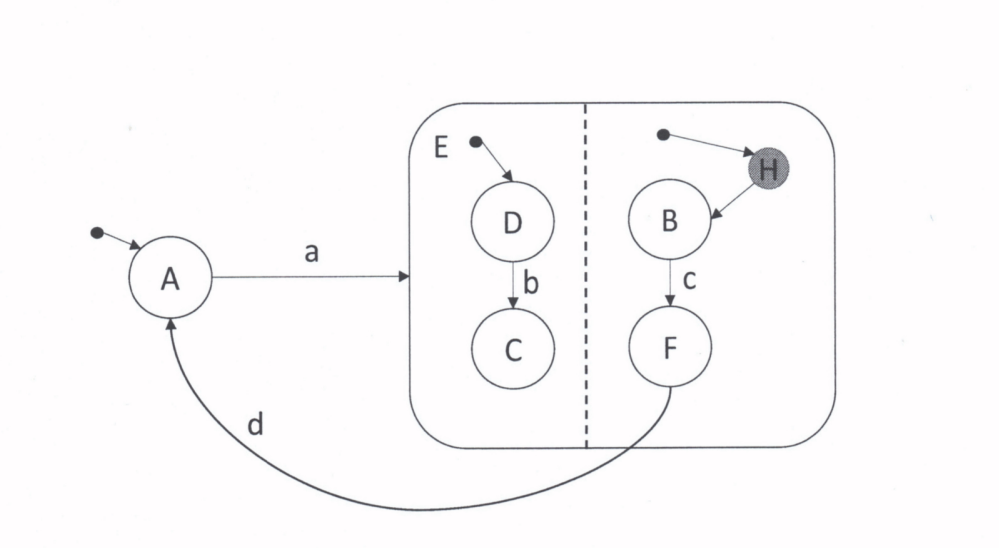
\includegraphics[width=10cm]{images/KA171121/5angabe.png}
  \centering
\end{figure}

\begin{figure}[H]
  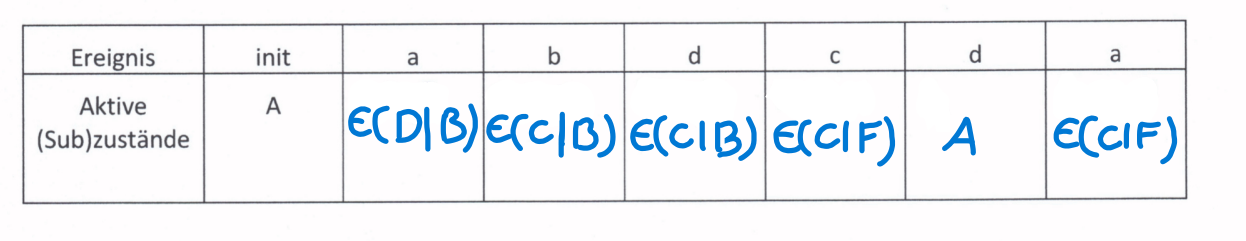
\includegraphics[width=10cm]{images/KA171121/5a.png}
  \centering
\end{figure}

\subsection{Speicherprogrammierbare Steuerung (SPS)}
In folgender Ablaufsteuerung werden drei Boolesche Variablen A, B und C verwendet die zu Beginn alle den Wert FALSE haben.

\begin{figure}[H]
  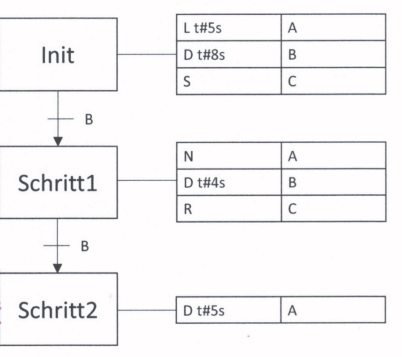
\includegraphics[width=10cm]{images/KA171121/6angabe.png}
  \centering
\end{figure}

A: $[0,5], [8,12], [17,\infty]$\\
B: $[8,8], [12,12]$\\
C: $[0,8]$